\chapter{Waveform Views}

A waveform view is a 2D graph of a signal or protocol decode within a waveform group.

\section{Navigation}

Scrolling with the mouse wheel adjusts the horizontal scale of the current waveform group, zooming in or out centered
on the position of the mouse cursor.

Pressing SHIFT while scrolling moves the view left and right without adjusting zoom. If your mouse has a horizontal
scroll feature, this may also be used to pan without zooming.

Pressing the middle mouse button auto-scales the active waveform group so that the entire waveform is visible.

\section{Plot Area}

The plot area shows the waveform being displayed. The background has a subtle gradient from light at top to dark at
bottom, in order to visually separate adjacent waveform view within the same group.

The horizontal grid lines line up with the voltage scale markings on the Y axis. If the plot area includes Y=0, the
grid line for zero is slightly brighter.

\begin{figure}[H]
\centering
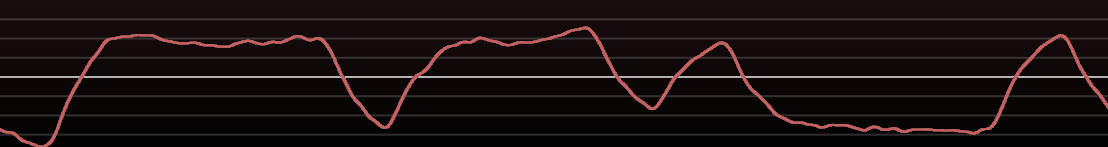
\includegraphics[width=10cm]{images/waveform-graph.png}
\caption{Waveform plot area}
\label{waveform-graph}
\end{figure}

The waveform is drawn as a semi-transparent line so that when zoomed out, the density of voltage at various points in
the graph may be seen as lighter or darker areas. This is referred to as ``intensity grading".

\begin{figure}[H]
\centering
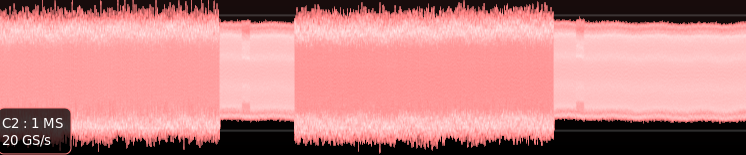
\includegraphics[width=10cm]{images/graded-waveform.png}
\caption{Intensity-graded waveform}
\label{graded-waveform2}
\end{figure}

\section{Y Axis Scale}

Each waveform view has its own Y axis scale, which is locked to the ADC range of the instrument.

Channel gain may be configured by scrolling with the mouse wheel, and offset may be adjusted by dragging with the left
mouse button. If the view is displaying the output of a filter block, you may use the middle mouse button to auto-scale
the vertical axis to the range of the current waveform. The auto-scale feature is not available for physical instrument
inputs.

If a left-pointing arrow (as seen in Fig. \ref{y-axis}) is visible, the current channel is selected as a trigger
source. Click on the arrow and drag up or down to select the trigger level. Some trigger types, such as window triggers,
have two arrows for upper and lower levels.

\begin{figure}[H]
\centering
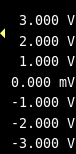
\includegraphics[height=3cm]{images/y-axis.png}
\caption{Y axis of a waveform view showing trigger arrow}
\label{y-axis}
\end{figure}

\section{Channel Information Box}

The channel information box is displayed in the lower left corner of each waveform view. It contains summary
information about the channel. Currently this is the display name of the channel, the sample rate, and the record
length of the acquisition. Other information, such as probe coupling, may be displayed there in the future.

\begin{figure}[H]
\centering
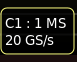
\includegraphics[width=2cm]{images/channel-infobox.png}
\caption{Channel information box}
\label{channel-infobox}
\end{figure}

The information box may be dragged with the left mouse button to move the entire waveform view to a new location.

Double-clicking the information box opens the channel properties dialog (Fig. \ref{channel-properties}). This dialog
allows changing of the channel's nickname or color. The ``hardware name" of the channel is also displayed, so that a
renamed channel can be easily traced back to a physical instrument input.

Depending on the particular instrument in question, other settings may be displayed here, such as fine deskew,
attenuation, polarity inversion, and bandwidth limiting. An input mux selector is shown if the scope has more than one
input per channel (such as the Teledyne LeCroy SDA and WaveMaster series).

The channel properties dialog also allows setting threshold and hysteresis for digital channels, and ADC configuration
for scopes that have variable analog resolution (such as the Teledyne LeCroy HDO9000 or Pico Technology 6000E series).
These settings are listed under channel properties since some instruments support per-channel adjustment of them,
however it it is important to note that these settings apply to multiple channels (a bank or even the entire
instrument) in some cases. A list box under these settings shows the list of other channels, if any, that share the
same configuration.

\begin{figure}[H]
\centering
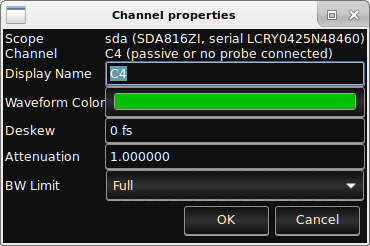
\includegraphics[width=8cm]{images/channel-properties.png}
\caption{Channel properties dialog}
\label{channel-properties}
\end{figure}

\section{Cursors}
\label{sec:cursors}

\subsection{Vertical Cursors}

To add a vertical cursor (Fig. \ref{vertical-cursor}), right click on the waveform and select \menustyle{Cursor |
Vertical (single)} or \menustyle{Cursor | Vertical (dual)} as appropriate.

\begin{figure}[H]
\centering
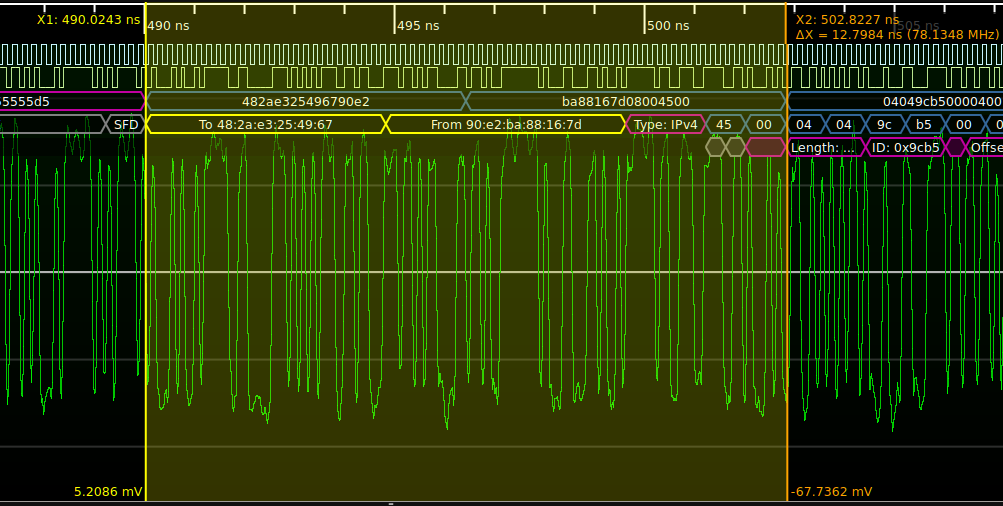
\includegraphics[width=13cm]{images/vertical-cursor.png}
\caption{Vertical cursor}
\label{vertical-cursor}
\end{figure}

To place a single cursor, click on the waveform at the desired location. To place double cursors, click at the starting
location to place the first cursor then drag to the ending location and release the mouse to place the second cursor.
Once placed, either cursor can be moved by clicking on it and dragging to the new location.

Cursors will snap to transitions in digital signals or protocol decode overlays if the mouse is within a few pixels of
the location. No snapping is applied when the mouse is over an analog waveform.

In the timeline each cursor will display its X-axis position. If both cursors are active, the delta between them
is shown. If the X axis uses time units, the frequency with period equal to the cursor spacing is also shown.

At the bottom of each waveform area, the Y-axis value of the signal where it crosses the cursor is shown. In FFT /
spectrum analyzer plots, the integrated in-band power between both cursors is also shown.

If a protocol analyzer view (Chap. \ref{chapter:protoanalyzer}) is active, moving a single cursor over a packet will
scroll to and highlight that packet.

\subsection{Horizontal Cursors}

To add a horizontal cursor (Fig. \ref{horizontal-cursor}), right click on the waveform and select \menustyle{Cursor |
Horizontal (single)} or \menustyle{Cursor | Horizontal (dual)} as appropriate.

\begin{figure}[H]
\centering
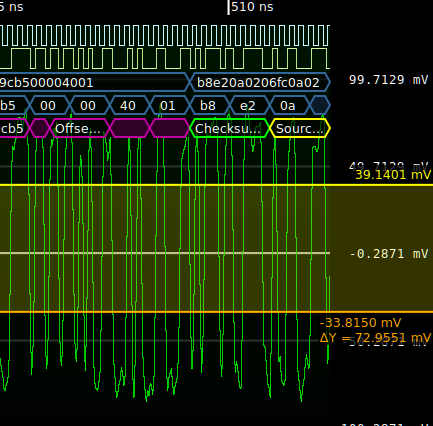
\includegraphics[width=8cm]{images/horizontal-cursor.png}
\caption{Horizontal cursor}
\label{horizontal-cursor}
\end{figure}

To place a single cursor, click on the waveform at the desired location. To place double cursors, click at the starting
location to place the first cursor then drag to the ending location and release the mouse to place the second cursor.
Once placed, either cursor can be moved by clicking on it and dragging to the new location.

At the right side of the plot, each cursor will display its Y-axis location. If both cursors are active, the delta
between them is also shown.

All waveform areas in a group share the same Y axis cursor positions.

\section{Overlays}

Waveforms may have additional information overlaid on top of them, such as protocol decodes. Each overlay has its own
information box, which may be double-clicked to open the properties dialog and configure it just like any other
channel.

Fig. \ref{overlays} shows an example of an analog waveform with five overlays: a CDR PLL, thresholding, and decodes of
the 64/66b line code, the 10Gbase-R Ethernet framing, and IPv4 packet headers.

\begin{figure}[H]
\centering
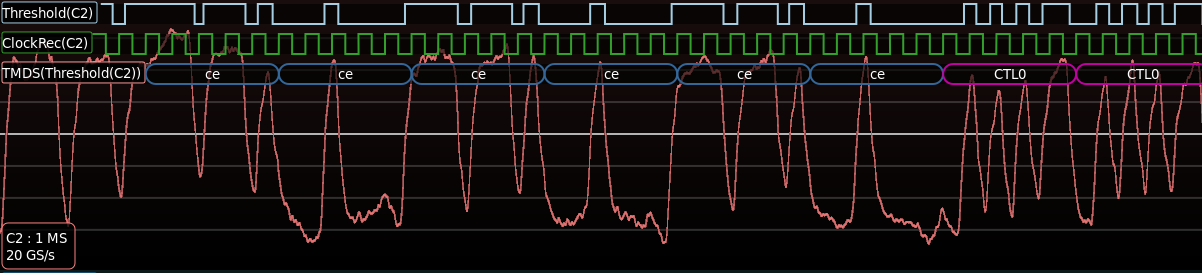
\includegraphics[width=14cm]{images/overlays.png}
\caption{Waveform showing two digital overlays and a three decode overlays}
\label{overlays}
\end{figure}

Overlays can be deleted by means of the right-click context menu. Dragging the information box with the left mouse
button allows overlays to be reordered, however they cannot currently be moved to another waveform view.

\section{Statistics}

Statistics (Fig. \ref{stats}) may be shown for any waveform by checking the ``statistics" box in the context menu. The
default statistics are minimum, average, and maximum although more may be added in the future.


\begin{figure}[H]
\centering
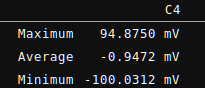
\includegraphics[width=5cm]{images/stats.png}
\caption{Statistics for an analog waveform}
\label{stats}
\end{figure}
